\section{Small Dynamic Subsystem Interface Protocol Architecture}
\label{sec:sdsip}

The Small Dynamic Subsystem Interface Protocol (SDSIP) is, as the name implies, a standardized
method of communication between subsystems. That is, the protocol is not limited to
avionics\footnote{Although
the focus of its implementation in this work being on an avionics system}. Its design is meant to
focus on generating interfaces to SDSIP compatible drivers seamless as well as making transmitting
and receiving data from other subsystems simple. Similarly to before, the architectures will be
presented to fully describe the package.

The overall operational architecture of SDSIP is represented in
\autoref{fig:sdsip-operational-architecture}. It is a module of the ADC

\begin{figure*}[ht]
  \begin{center}
    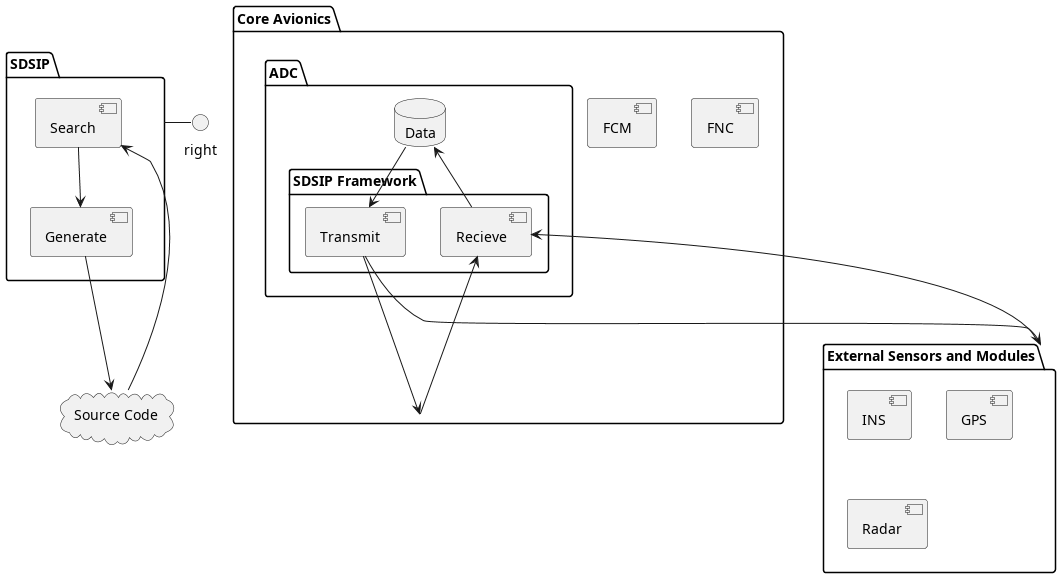
\includegraphics[width=0.90\textwidth]{sdsip-operational-architecture}
  \end{center}
  \caption{}
  \label{fig:sdsip-operational-architecture}
\end{figure*}
